% !TEX root = ../notes_template.tex
\chapter{Muscle Energetics}\label{chp:energetics}
Updated on \today
\minitoc

Muscles transform chemical energy into mechanical energy. The chemical energy utilized in this transformation is ATP. However ATP is not ingested and then circulated through the body to the cells. It is present in the cells in small quantities and regenerated in the cells at a rate that approximates its rate of utilization. The primary utilization ATP in the muscle cell for active tension occurs when it is hydrolyzed by myosin ATPase during crossbridge cycling. The change in shape of the myosin head is potential mechanical energy that becomes kinetic mechanical energy during crossbridge activation. Muscle excitation and activation requires ATP in two other key steps. The $Na^+ / K^+$-ATPase pumps to establish the resting membrane potential, and the $Ca^{2+}$-ATPase pumps to return $Ca^{2+}$ into the sarcoplasmic reticulum. Beyond these clear ATP needs for excitation, activation and tension the muscle fibers continually require ATP, even while at rest, for membrane transport and for synthesis of chemical compounds throughout the fiber that are critical for integrity (maintenance and adaptation). 
The chemical energy to regenerate ATP comes from food we ingest, digest, absorb and metabolize into substrates. Not all substrates require metabolism, but some sort of biochemical metabolic pathway is involved when anything other than glucose is used as the substrate (this includes the use of glycogen, a stored form of glucose).
This chapter considers the rate and capacity of five pathways to regenerate ATP in muscle cells. These five pathways vary across a spectrum with rate of regeneration inversely related to capacity. They are all always being utilized to some extent during muscle cell energetic transformations. Structural variations that exist on a spectrum between muscle fibers result in functional variation in their ability to carry out these five pathways with a high degree of adaptability. Clinical physiology connections emerge based on an understanding of energetics, this chapter will focus on the implications of sarcopenia, the concept of fatigue, and the pathophysiological concepts of hypoxia, hypoxemia and ischemia.

\vspace{5mm}

\textbf{Objectives include:}
\begin{enumerate}
    \item Explain the factors underlying the storage, use and regeneration of ATP.
    \item Explain the structure and function of energetic components of muscle fibers.
    \item Compare and contrast the energetic system pathways that transform macro nutrient substrates to ATP.
    \item Compare and contrast muscle fiber differentiation (types) based on energetic structures and resultant functional capacities.
    \item  Apply the concepts of mass balance, flow gradients, and energy to the analysis of patient/client problems related to the muscular system.
     \item Evaluate the different energetic pathways used in different activities, and analyze the response to different activities to energetic pathways.
     \item Explain the implications of sarcopenia on muscle strength and endurance.
     \item Explain the concept of, and the energetic basis of fatigue.
     \item Explain the energetic basis of hypoxia, hypoxemia and ischemia.
\end{enumerate}

\section{Energetic Transformation Overview}

Energetic Transformation is a slightly more explanatory way of describing what is commonly referred to as metabolism. Of course, there are many different types of energetic transformations occurring when considering all metabolism throughout the body. And not all metabolic reactions are specifically about the regeneration of ATP. Here we'll be focusing on metabolic processes and pathways in muscle that are utilized to regenerate ATP. However, most of these processes and pathways occur in cells throughout the body (actually, throughout the animal kingdom). 

Muscle fibers continuously require ATP. Despite how important ATP is to muscle fiber function, even at rest, it is maintained at relatively low concentrations (5 $mmol \cdot L^{-1}$) \cite{feher_quantitative_2017, jones_skeletal_2006}. For cells with a steady and relatively low energetic need the tendency for cells to store a small amount of ATP is not a problem. Even for muscles at resting metabolism it is not a problem. Unlike most cells the muscle fibers can increase their metabolic rate (rate of ATP regeneration through energetic transformation) 60-100 fold during transitions from rest to high levels of tension. Resting muscle has approximately 1 $mmol \cdot L^{-1}$ of ADP and 10 $mmol \cdot L^{-1}$ of $P_i$. One hypothesis of energetic transformation regulation is the ATP:ADP ratio, which is maintained at approximately 5:1.

There are two proposed reasons that ATP is not stored in large quantities. First, it is a heavy molecule. It is estimated that an individual regenerates their body weight worth of ATP. ATP is 507.18 g/mole. Whereas glucose is 180 g/mole and even fatty acids with up to 29 carbon chains and double bonds (high energy) have molar masses lower than ATP (<500 g / mole). Since mass (and weight) influence the energetic costs of movement then storing ATP is a much less efficient approach to energy storage than storing glucose (such as glycogen) and fatty acids (as adipose tissue). Second, ATP is a highly reactive molecule that can trigger several cellular events by binding and hydrolyzing. One source refers to the situation of too much ATP being stored as causing "chaos" to cellular functions \cite{jones_skeletal_2006}. The implications of not storing ATP includes the continuous need to regenerate ATP at the rate that it is being utilized with a small amount of reserve or surge capacity.



\section{ATP Regeneration Pathways}

Overall there are six ATP regeneration pathways in the muscle fiber. The myokinase pathway is briefly described as part of the immediate ATP/Phosphocreatine (PCr) pathway. The pathways are summarized in Figure \ref{fig:Energetics_Overview}. The rates and capacities of the pathways are later directly compared in Table \ref{table:ATP_Rates}. 


\begin{figure}[!h]
    \centering
    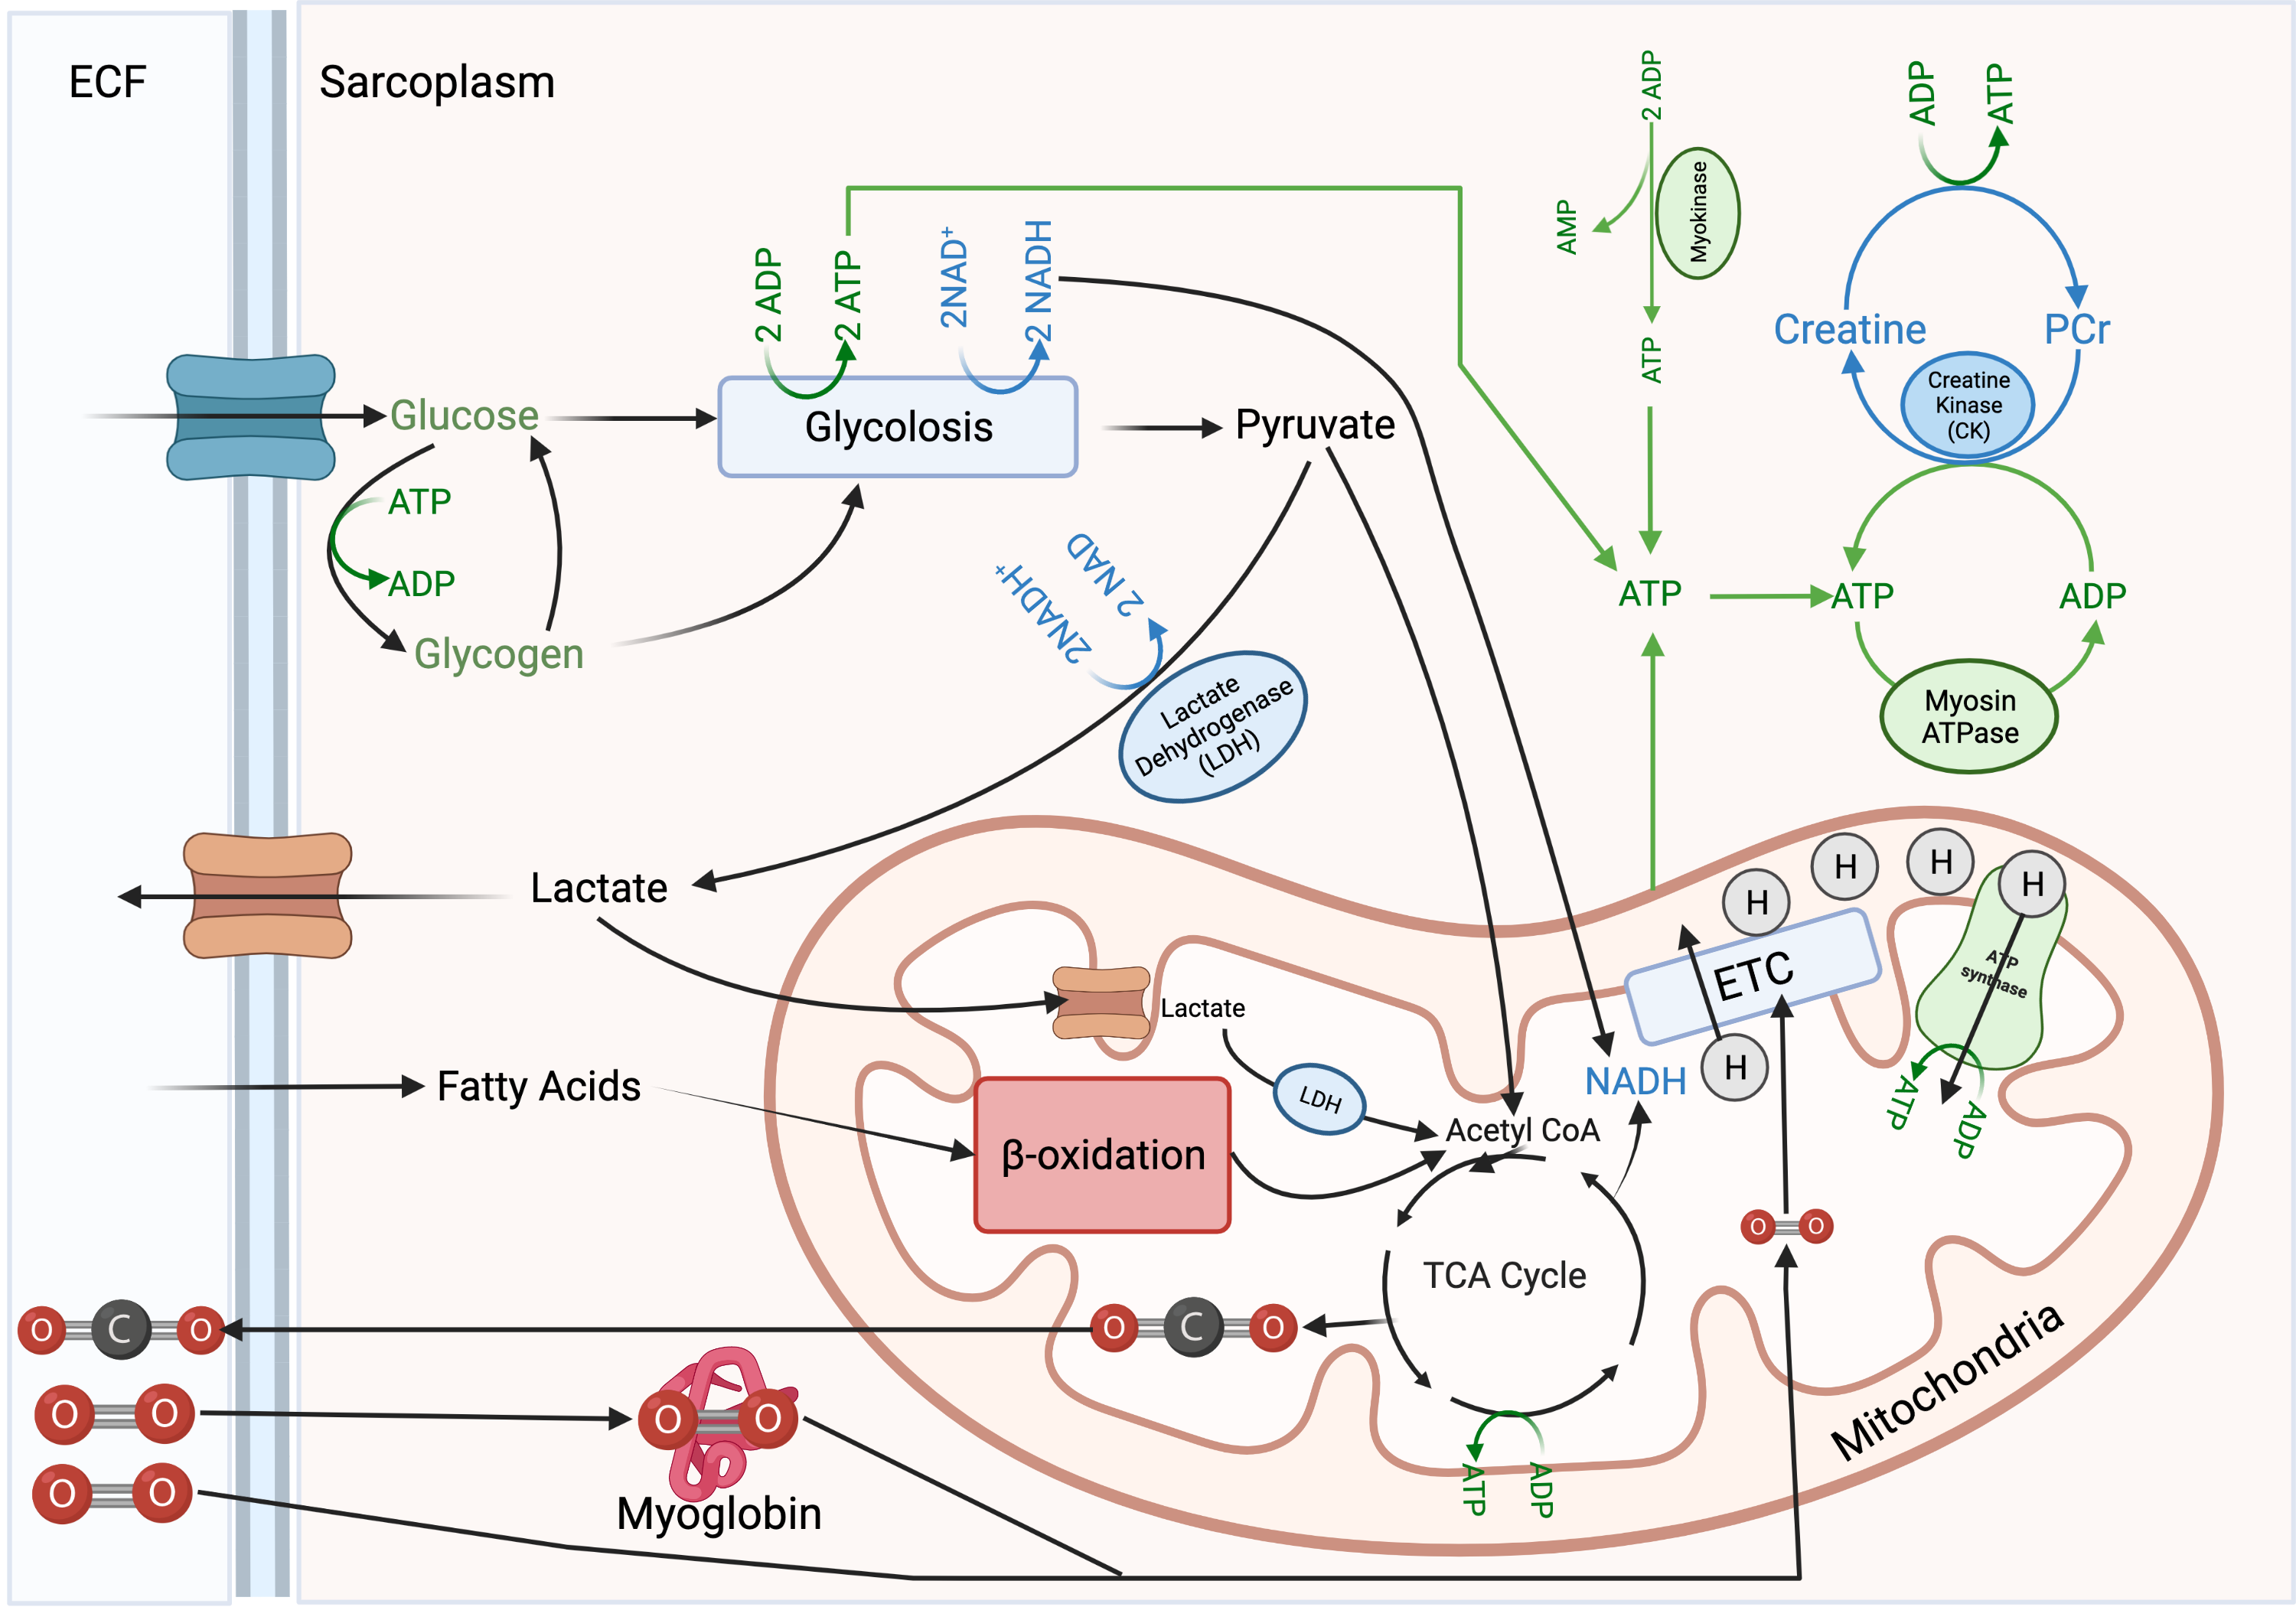
\includegraphics[width=1\linewidth]{./figure/Energetics_Overview.png}
    \caption{Overview of Energetic Transformation Pathways in a Muscle Fiber. The only pathway not explicitly included in this graphic is the pathway that starts with the breakdown of glycogen to release glucose into the blood which ultimately enters cells through the glut4 channel. This and other important metabolic processes and pathways in the liver are covered in Chapter \ref{chp:blood_nutrients}. (\footnotesize{Created with BioRender.com})}
    \label{fig:Energetics_Overview}
\end{figure}

Some of the pathways occur in the sarcoplasm (outside of the mitochondria, including PCr, Myokinase, Muscle Glycogen $\rightarrow$ Lactate Pathway). These pathways are not rate limited by the structural requirements of mitochondria.  Pathways occurring outside of the mitochondria do not involve cellular respiration and can be referred to as anaerobic (not requiring O2). The anaerobic pathways follow standard chemical substrate phosphorylzation. The chemical reactions of these pathways are catalyzed (expedited) by enzymes and produce ATP at high rates but low overall yield. The low yield is due to the fact that they tend to be self limiting. They either recycle existing energy and quickly exhaust their capacity (myokinase and PCr) or they create byproducts that inherently limit their process (the glycolytic process within the Muscle Glycogen $\rightarrow$ Lactate pathway). With either self limitation they produce ATP at a higher rate than their support systems allow. They meet a particular need, provide a high rate of ATP regeneration, but fatigue quickly and must recover. Such work:recovery cycles are a recurring theme for the concept of fatigue.

Pathways occurring in the mitochondria involve cellular respiration and are referred to as aerobic (Muscle Glycogen $\rightarrow$ $CO_2$; Liver Glycogen $\rightarrow$ $CO_2$; Fatty Acid $\rightarrow$ $CO_2$ pathways). Any pathway that produces Acetyl Co-A can enter into the Citric Acid Cycle (TCA, Kreb's Cycle). TCA contributes some ATP, but primarily contributes more NADH+ and creates some CO2 in the process. NADH+ is utilized to generate large quantities of ATP by sending it through the Electron Transport Chain (ETC). The ETC utilizes NADH+ to build a concentration and electrochemical gradient of H+ in the inner membrane, an process which is rate dependent on the availability of O2 to accept the electrons that have been transported. The energy of this gradient is then pushed through ATP-synthase much like water through a turbine at a dam. One of the reasons there are fluctuating estimates on the number of ATP produced through these aerobic pathways (oxidative phosphorylation) is that the ATP is produced by the function of a molecular machine, not with standard chemical substrate phosphorylzation. 

% No switch - all of the biochemical pathways are occuring at the same time, the flux through each is dependent on the need for ATP and that need is based on the need for energy. High metabolism refers to the situation of needing more ATP. The entire system of using $O_2$ consumption as a biometric of metabolism is predicated on the ultimate use of $O_2$ to energize all ATP. Even when PCr is used to energize a muscle activation the creatine (Cr) is ultimately regenerated (PCr) by an ATP 

\paragraph{There is no switch!}
There is no switch that turns on anaerobic energy transformation and turns off aerobic; or that turns on aerobic or off anaerobic. There are no exercises that are exclusively anaerobic or exclusively aerobic. A slow walk in a health individual still utilizes what could be considered anaerobic pathways. A heavy lifting session regenerates ATP and PCr between sets utilizing aerobic pathways. Dispel any notions in your brain that these socially constructed concepts entail an exclusive monopoly of energetic pathways to regenerate ATP. All energetics are on a spectrum and at best the primary demand for ATP during the slow walk are met by aerobic pathways, and the primary demands of the heavy lifting session are met by anaerobic pathways (ultimately regenerated by aerobic metabolism). It is this concept of meeting primary demands that has been utilized for the social construction of aerobic and anaerobic exercise and the misinterpretation that these are mutually exclusive pathways.

\paragraph{There is no ATP Debt}

There is no such thing as ATP dept. ATP is needed for cellular functions. Either the pathways provide a way to regenerate the ATP needed for the demand, or the cellular functions do not occur.


\subsection{ATP / Phosphocreatine (PCr) (immediate) Pathway}

% Include the concept of diffusion of ATP through the muscle cell and the hypothesized use of PCr to facilitate the transport of ATP through the sarcoplasm

Creatine is synthesized in the liver, or ingested, digested and then absorbed from meat or ingested and absorbed from supplementation.\footnotemark\footnotetext{Creatine is a molecule that can be absorbed directly through the gut into the blood. Creatine supplementation will be a clinical connection in Chapter \ref{chp:blood_nutrients} on Visceral Support.} A high energy bond can form between creatine and phosphorous ($P_i$), forming PCr.

The reaction: $PCr \rightleftharpoons ATP$ is a reversible high rate reaction catalyzed by the enzyme creatine kinase (CK). The rightward reaction (PCr to ATP) regenerates ATP for cellular functions. At rest about 80\% of creatine is in the energized (PCr) state and there is approximately five times as much PCr than ATP (PCr:ATP ratio of 5:1). Based on the weight and reactive volatility of ATP, PCr is provides a very important reserve of high energy phosphate bonds for ensuring the muscles ability to meet high energy demands, and even to smooth out transitions between lower and higher ATP utilization rates.\footnotemark\footnotetext{As a reminder, the primary determinant in a muscle fiber of ATP utilization is the frequency of activation which is directly proportional to frequency summation.} It is a stable and relatively light form of energy to store in the muscles.

PCr is considered an immediate source of ATP and the flux rate of PCr to ATP is determined by the ATP:ADP ratio. As ADP levels increase the rate of PCr to ATP reactions increase and will continue until PCr is expended or ADP drops to a normal level.

The maximum rate of $PCr \rightleftharpoons ATP$ is much higher than other pathways, upwards of 4.4 moles/minute of ATP. However, it is only capable of regenerating approximately 0.7 moles of ATP overall. Therefore, when working at maximum capability (rate of 4.4 moles/minute) it would only be sustained for 9.5 seconds (See the Summary of Max Rates of ATP Regeneration by Pathway in Table \ref{table:ATP_Rates}. This time estimate is dependent on the assumption of the max rate (4.4 moles/minute). Once the capacity of PCr to regenerate ATP is exhausted (fatigued) the muscle will not be able to continue to generate a tension that requires that rate of ATP utilization.

If a lower rate of ATP was being utilized, say .5 moles/minute, then PCr would be able to sustain ATP regeneration much longer. And if that rate of ATP utilization was lower than other pathways then PCr would continue, itself, to be regenerated and the need for ATP from PCr would not approach maximum because other pathways would be contributing to the ATP need.

Even though PCr is most often thought of as the source of ATP for high muscle tension activities, it also is the initial source of ATP for any changes in the rate of utilization of ATP because other pathways have a delay (when compared to PCr) in how quickly they can start regenerating more ATP. Therefore, PCr is the source of ATP for a sudden burst of tension such as that needed to increase pace during a run, or increase velocity of a movement.

\paragraph{ATP-PCr Sarcoplasm Shuttle}
The PCr pathway is hypothesized to be utilized as a ATP transport mechanism throughout the sarcoplasm (ATP-PCr shuttle). There are substantial diffusion barriers in a muscle fiber due to the number of highly structured protein complexes. The mitochrondria are near the sarcolemma (along with the nuclei largely because the rest of the fiber is packed tightly with myofilaments) and thus the diffusion of ATP from the mitochrondria to myosin-ATPase is challenging. PCr is diffused through the entire sarcoplasm and due to its rapid regeneration rate can easily shuttle (or pass) the energy of ATP through the sarcoplasm from just outside a mitochondria to near the myosin ATPase. During muscle activation when the rate of ATP use by the myosin ATPase increases the nearby PCr regenerate ATP and then that regeneration can propagate from all around the sarcoplasm, and from near the mitochondria, to shuttle ATP toward the myosin ATPase (See Figure \ref{fig:PCr}). This movement - either the diffusion of ATP directly or the use of an ATP-PCr shuttle is based on the flow gradient. The more ATP being utilized by the myosin ATPase, the $Na^+/K^+$-ATPase or the $Ca^{2+}$ ATPase the lower the concentration of ATP near those proteins and the greater the diffusion, and shuttling, of ATP towards those locations.

\begin{figure}[h!]
    \centering
    \includegraphics{}
    \caption{Movement of ATP through the sarcoplasm using an ATP-PCr shuttle}
    \label{fig:PCr}
\end{figure}

\paragraph{Myokinase (Adenylate Cyclase)}

Another "immediate" high rate reaction to regenerate ATP is the myokinase (enzyme, also referred to as adenylate cyclase) that catalyzes the reaction: $2ADP \rightleftharpoons AMP + ATP$. During this reaction a $P_i$ is hydrolyzed from ADP and the energy is utilized to regenerate ATP. While this reaction can happen at a high rate, it is limited and probably only utilized in extreme "ATP need" situations. In such situations this reaction allows continued cell functions for a short period of time. Estimates are that under conditions of maximum ATP utilization (upwards of 4.4 moles/minute), this system could be sustained for milliseconds. For our purposes it is therefore added to the ATP/PCr row of Table \ref{table:ATP_Rates} given its relatively insignificant contribution.

\subsection{Muscle Glycogen $\rightarrow$ Lactate Pathway}

The muscle glycogen (or glucose) $\rightarrow$ lactate pathway provides ATP regeneration at a moderate rate. It is only capable of maximum rates for a relatively small amount of ATP and therefore for a short period of time. The key biochemical process for this pathway is glycolosis. 
Glycolosis transforms glucose or glycogen into several important end products including ADP to ATP, NAD to NADH and pyruvate. When regenerating ATP at high rates glycolosis ends up creating more NADH and there is not enough NAD to continue with glycolosis, and the accumulation of NADH results in a drop in intracelluar pH. As a remedy to this situation NADH is converted back into NAD which includes the conversion of pyruvate into lactate.

So the glycogen (or glucose) $\rightarrow$ lactate pathway, while always involved a bit, is primarily involved when it is functioning at a rate of ATP regeneration that exceeds the ability of the muscle glycogen $\rightarrow$ $CO^2$ pathway. Based on the estimates in Table \ref{table:ATP_Rates}, if the glycogen (or glucose) $\rightarrow$ lactate pathway is generating over 1 mole / minute of ATP it is exceeding the rate that the muscle glycogen $\rightarrow$ $CO^2$ pathway. In this situation it is beneficial to the muscle fiber for lactate to form and be shuttled out of the cell to stabilize the pH and to make NAD available to continue glycolosis. 

If the glycogen (or glucose) $\rightarrow$ lactate pathway towards lactate continues it eventually cannot shuttle lactate out of the cell fast enough and cellular pH drops (acidity), and there is not enough NAD, so the rate of glycolosis slows down (forcing a recovery period). A consequence for the muscle is that it cannot continue to generate tension at a rate that requires such a high rate of ATP regeneration.

\paragraph{Anaerobic Threshold - Lactate Threshold - Onset of Blood Lactate Accumulation}
Anaerobic threshold (AnT), lacate threshold (LT) and onset of blood lactate accumulation OBLA) are three related concepts. AnT is primarly theoretical and can be estimated by LT or OBLA which are both measurements of blood lactate. Ventilatory threshold (VT) is another approach to measuring AnT discussed in Chapter \ref{chp:fick_equation}. The concept of AnT is directly related to the previously discussed idea that when the glycogen (or glucose) $\rightarrow$ lactate is regenerating ATP at a rate higher than capable by the glycogen (or glucose) $\rightarrow$ $CO^2$ pathway, the pH of the cell drops and an increased amount of lactate is shuttled out of the cell into the blood.

% Stopped here

\subsection{Muscle Glycogen $\rightarrow$ $CO_2$ Pathway}

If $CO_2$ is created it is cellular respiration as part of the citric acid cycle (TCA). $O_2$ is consumed as part of the electron transport chain (ETC). Note that $CO_2$ is produced and $O_2$ is consumed at different steps in the pathways that produce $CO_2$ a byproduct and consume $O_2$.

$CO_2$ produced as part of TCA (also referred to as Kreb's cycle)
$O_2$ consumed as part of ETC (also referred to as oxidative phosphorylation)
TCA and ETC combined can be referred to as oxidative metabolism. 

Even though the $CO_2$ production and the $O_2$ consumption does not occur at the same steps in the pathways, whenever you see that $CO_2$ is produced, you can assume that $O_2$ is being consumed. 

\subsection{Liver Glycogen $\rightarrow$ $CO_2$ Pathway}

\subsection{Fatty Acids $\rightarrow$ $CO_2$ Pathway}



Mitochondria Extract Energy From Nutrients (p. 24) The principal substances from which the cells extract energy are oxygen and one or more of the foodstuffs—carbohydrates, fats, and proteins—that react with oxygen. In humans, almost all carbohydrates are converted to glucose by the digestive tract and liver before they reach the cell; similarly, proteins are converted to amino acids, and fats are converted to fatty acids. Inside the cell, these substances react chemically with oxygen under the influence of enzymes that control the rates of reaction and channel the released energy in the proper direction.

Mitochondria Extract Energy From Nutrients (p. 24) The principal substances from which the cells extract energy are oxygen and one or more of the foodstuffs—carbohydrates, fats, and proteins—that react with oxygen. In humans, almost all carbohydrates are converted to glucose by the digestive tract and liver before they reach the cell; similarly, proteins are converted to amino acids, and fats are converted to fatty acids. Inside the cell, these substances react chemically with oxygen under the influence of enzymes that control the rates of reaction and channel the released energy in the proper direction.
Oxidative Reactions Occur Inside the Mitochondria, and Energy Released Is Used to Form ATP ATP is a nucleotide composed of the nitrogenous base adenine, the pentose sugar ribose, and three phosphate radicals. The last two phosphate radicals are connected with the remainder of the molecule by high-energy phosphate bonds, each of which contains about 12,000 calories of energy per mole of ATP under the usual conditions of the body. The high-energy phosphate bonds are labile so they can be split instantly whenever energy is required to promote other cellular reactions. When ATP releases its energy, a phosphoric acid radical is split away, and adenosine diphosphate (ADP) is formed. Energy derived from cell nutrients causes ADP and phosphoric acid to recombine to form new ATP, with the entire process continuing over and over again. Most of the ATP Produced in the Cell Is Formed in Mitochondria After entry into the cells, glucose is subjected to enzymes in the cytoplasm that convert it to pyruvic acid, a process called glycolysis. Less than 5\% of ATP formed in the cell occurs via glycolysis. Pyruvic acid derived from carbohydrates, fatty acids derived from lipids, and amino acids derived from proteins are all eventually converted to the compound acetyl coenzyme A (acetyl-CoA) in the mitochondria matrix. This substance is then acted on by another series of enzymes in a sequence of chemical reactions called the citric acid cycle, or Krebs cycle. In the citric acid cycle, acetyl-CoA is split into hydrogen ions and carbon dioxide. Hydrogen ions are highly reactive and eventually combine with oxygen that has diffused into the mitochondria. This reaction releases a tremendous amount of energy, which is used to convert large amounts of ADP to ATP. This requires large numbers of protein enzymes that are integral parts of the mitochondria. The initial event in ATP formation is removal of an electron from the hydrogen atom, thereby converting it to a hydrogen ion. The terminal event is movement of the hydrogen ion through large globular proteins called ATP synthetase, which protrude through the membranes of the mitochondrial membranous shelves, which themselves protrude into the mitochondrial matrix. ATP synthetase is an enzyme that uses the energy from movement of the hydrogen ions to convert ADP to ATP, and hydrogen ions combine with oxygen to form water. The newly formed ATP is transported out of the mitochondria to all parts of the cell cytoplasm and nucleoplasm, where it is used to energize the functions of the cell. This overall process is called the chemiosmotic mechanism of ATP formation.



\subsubsection{Pathways for Protein Energetics}

There are a variety of pathways for protein energetics, but they are not an optimal source of energy and not the best use of protein. The pathways are reserved for extreme situations. These pathways involve protein breakdown into amino acids and the use of amino acids at various steps of other pathways (requires removal of nitrogen), or in the liver during gluconeogenesis. Gluconeogenesis is the generation of glucose from non carbohydrate carbon sources including amino acids (amongst other molecules such as lactate, pyruvate, acetyl-CoA and fatty acids).


\subsection{Rates and Capacities}

Rates and capacities of ATP regeneration for each of the pathways are included in Table \ref{table:ATP_Rates}.

\begin{table}[h!]
\centering
\begin{tabular}{||c c c c||} 
 \hline
Source & Max Rate of ATP (mol/min) & Amount of ATP (mol) & Time at Max (s or min)\\ [0.5ex] 
 \hline\hline
 ATP/PCr/Myokinase & 4.4  & 0.7 & 9.5 s \\
 Muscle Glycogen $\rightarrow$ Lactate &  2.4 & 1.6 & 40 s \\ 
 Muscle Glycogen $\rightarrow$ $CO_2$ & 1.0 & 84 & 84 min\\
 Liver Glycogen $\rightarrow$ $CO_2$  & 0.4 & 19 & 48 min \\ 
 Fatty Acids $\rightarrow$ $CO_2$ & 0.4 & 4000 & 10,000 min \\[1ex] 
 \hline
\end{tabular}
\caption{Summary of Max Rates of ATP Regeneration by Pathway (\footnotesize{Data from \cite{feher_quantitative_2017}})}
\label{table:ATP_Rates}
\end{table}

When considering the time estimates based on the quantity of ATP can be be regenerated by various energetic pathways it is important to consider that two factors influence the sustainability of the pathway. First whether the pathway, at its max rate, is rate limiting. Second, the availability of the substrate (macro-nutrients) in storage. Another consideration for the time estimates in Table \ref{table:ATP_Rates} is that the times are calculated based on the assumption of the max rate. For example, the 10 second estimate for ATP/PCr (which is a commonly cited estimate for this system) is entirely predicated on the max rate of ATP regeneration from ATP/PCr, which is based on the demand for ATP by the muscle. If the demand for ATP by the muscle is 2.2 mol/min then the time that ATP/PCr could contribute would be approximately 19 seconds. If the demand for ATP by the muscle is 1.1 mol/min then the time that ATP/PCr could contribute would be approximately 38 seconds. By this time the Muscle Glycogen $\rightarrow$ $CO_2$ pathway could be contributing and meeting most of the ATP demand of the muscle. 





\begin{table}[h!]
\centering
\begin{tabular}{||c c c c||} 
 \hline
Events & Rate of ATP Consumption (mol/min) & Amount of ATP (mol) & Estimated Time (s or min)\\ [0.5ex] 
 \hline\hline
 Rest & 0.12  & 173 & One Day \\
 100 Meter Sprint & 2.8 & 0.5 & 10 seconds \\ 
 800 Meter Run & 2.0 & 3.4 & 192 seconds\\
 1500 Meter Run & 1.7 & 6 & 210 seconds \\ 
 42,0000 Meter Run & 1.0 & 150 & 150 minutes \\[1ex] 
 \hline
\end{tabular}
\caption{Estimated Rate of ATP Consumption during Various Timed Running Events (\footnotesize{Data from \cite{feher_quantitative_2017}. Resting data is estimated based on basal energy expenditure of 1200 calories, and a conversion rate of about 6.93 calories per mole of ATP.})}
\label{table:Event_ATP_Rates}
\end{table}


\section{Motor Unit \& Muscle Fiber Types}

\begin{table}[h!]
\centering
\begin{tabular}{||c c c c c||} 
 \hline
 Muscle Fiber Type & Mitochondria & Myoglobin & Glycolytic Enzymes & PCr \\ [0.5ex] 
 \hline\hline
 Fast Glycolytic (FG)  & + & + & +++ & +++ \\ 
 Fast Oxidative Glycolytic (FOG) & ++ & ++ & ++ & ++ \\
 Slow Oxidative (SO) &  +++ & +++ & + & + \\ [1ex] 
 \hline
\end{tabular}
\caption{Energetic Characteristics of Muscle Fiber Types}
\label{table:Muscle_Fiber_Energetics}
\end{table}

\subsection{Slow Oxidative (S/SO/Type 1}

\subsection{Fast Oxidative Glycolytic (FR/FOG/Type 2x}

\subsection{Fast Glycolytic (FF/FG/Type 2a}




\section{\textit{Clinical Physiology Connections}}

\subsection{Sarcopenia}

Sarcopenia is an age related loss of muscle fibers with a bias toward FG fibers (FF motor units). A consequence of sarcopenia is a loss of the ability to attain the upper ranges of muscle tension. Expected consequences are a reduction in peak tension, high forces and high velocities of movement. An unexpected, paradoxical, consequence is a reduction in the ability to sustain lower ranges of muscle tension. This paradoxical consequence is based on the need to recruit the remaining motor units with increased frequency to meet the tension requirements of movement. Recruiting an S motor unit and its SO fibers more frequently (frequency summation) requires a higher rate of ATP than can be sustained. There is no question that S motor units and SO muscle fibers can achieve a higher rate of ATP than FF motor units and FG muscle fibers. But at a high level of tension (relative to the motor units capacity) the higher rate of crossbridge activation requires a higher rate of ATP regeneration. If that higher rate of ATP regeneration is greater than the rate capacity of the Glycolosis $\rightarrow$ $CO_2$ pathway, then the fiber will need to utilize the Glycolosis $\rightarrow$ Lactate pathway, which is self limiting (cannot be sustained). 

Let's walk through it with a simple model example. Assume walking requires 50\% output (tension) of 1/4 of the motor units. At this output the fibers require 0.7 moles of ATP / minute. In this scenario the Glycolosis $\rightarrow$ $CO_2$ pathway is sufficient and the activity is sustainable. Now assume there has been a loss of motor units. Now there are 1/2 of the prior motor units, and they are predominantly lower tension generating (S/SO) because the loss (due to sarcopenia) results in a loss of FG/FOG muscle fibers. Now walking (at the same pace as before) requires 75\% output from 3/4 of the fibers (since a twitch generates less tension there needs to be more frequency and motor unit summation). At this output the fibers require 1.3 moles of ATP / minute. In this scenario the Glycolosis $\rightarrow$ $CO_2$ pathway is not sufficient and the Glycolosis $\rightarrow$ Lactate pathway must be utilized to supplement ATP regeneration, which is not sustainable. Continuing to walk at this pace will result in fatigue. That is the paradoxical consequence of the loss of FF motor units in sarcopenia. Everyone expects a loss in the ability to attain tension (as measured by peak force). But there is also a loss in the ability to sustain tension (as measured by the ability to continue developing tension for an activity).


\subsection{Fatigue}

% Robustness (surge capability) - sensing the reserve
% Fidelity - objective (outward) 
% Efficacy - subjective (inward - how am I doing this act, how is it being supported?)
% Integrity - you need the reserve, so don't completely exhaust it / use it
% Fatigue - roll up, signal, regarding sustaining (and then can't attain what you started with)

Biological systems include cycles. Ca+ is released and taken in, muscle fibers develop active tension and then they don't, movements happen then they don't, we are awake and then asleep, etc. Across all scales in biological systems there are cycles. These cycles include spending resources, capabilities, and reserves and then building them back up. The concept of fatigue is fundamentally about these cycles. At the most general level fatigue occurs when resources, capabilities and reserves have been utilized and it is time for the cycle to be completed and go to its next phase (work to rest for example). If the cycle leading to fatigue is not completed, then fatigue occurs.

Fatigue is a pervasive concept because it can be applied to any aspect of a system with cycles occurring at any scale, which is any system doing an act, which is any system. Reading about fatigue is sure to result in several different interpretations. Muscle fatigue is the inability continue to sustain a tension with repeated excitation, and with fatigue the inability to attain a previously attainable tension. Running fatigue is the inability to sustain a pace with continued running, and the inability to attain that pace until recovery has occurred. Chronic fatigue syndrome is characterized by a severe lack of energy following exertions. The word fatigue can be like the description of the elephant by blind monks in Figure \ref{fig:elephant}. One monk describes the elephant as like a rope (while feeling the tail), another like a snake (while feeling the trunk), another like a wall (while feeling the body), another like a tree trunk (while feeling a leg), another like a spear (while feeling the tusk), and another like a large sheet (while feeling the ear).    

\begin{figure}[!h]
    \centering
    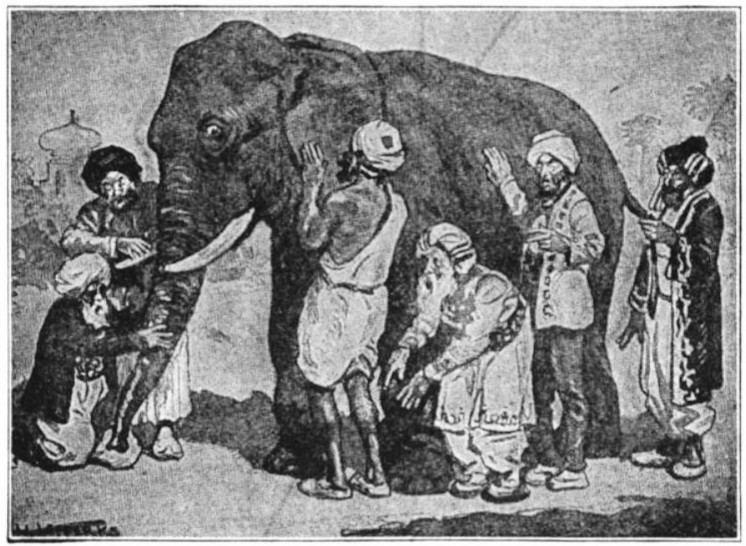
\includegraphics[width=1\linewidth]{./figure/elephant.jpg}
    \caption{Five Blind Monks Describing an Elephant (\footnotesize{Public Domain from \href{https://commons.wikimedia.org/wiki/File:Blind_men_and_elephant.png}{Sophie Woods, World Stories for Children, Ainsworth & Co. (Chicago), p. 14}})}
    \label{fig:elephant}
\end{figure}

of a system at any scale with one meaning, two perspectives and many applications. The one meaning of fatigue is an inability of a system\footnotemark\footnotetext{In our case a biological system.} to accomplish its act. It represents a failure to achieve act objectives. Note that this meaning is objective. The fact that the act cannot achieve its objective is measurable in some way. So the meaning of fatigue and the objective perspective are coherent. 

The subjective perspective, at least in terms of human fatigue, is the feeling (perception) of fatigue. Sometimes people confuse the subject and the objective. Notice again that the objective perspective of fatigue includes the inability of the system to achieve its act based on some measurable objective. If the system is meeting the objective of its act then it is not fatigued. However, there may be a perception of fatigue, and the person can report that they are fatigued. Both need to be considered and both pieces of information are important. For example, if a person walking 4 mph on a treadmill starts to feel fatigued during this act but they can accomplish the act then they are not objectively fatigued (they are doing the act), but they are subjectively feeling fatigued (or perhaps tired; or out of breath which can be confused symptomatically with fatigue). The new symptom of (perception of) fatigue in this individual despite being able to meet the objective of the act means that the person is not fatigued for the act of walking at the point they are doing the walking. But that perception is probably arising because some supporting system for that act of walking is fatigued and perhaps in an objective measurable (but not currently measured) act. That failure results in the need for other support systems to provide more support than usual to the walking act. Whether the fatigue in these support system can compensate or not, whether they are sustainable or not, influences whether and if so how long the walking act at 4 mph can continue. Once all possible support systems are fatigued then the walking act will no longer be able to continue at 4 mph, so the person slows down the treadmill to 3 mph and they are doing a new act that they can possibly continue. At this new walking act, the energetic requirements may be low enough that all of the support systems recover to full capability and the person can go back to 4 mph for a time being. The change in the ability - previously being able to do 4 mph without fatigue to now not being able to do 4 mph without fatigue - can be due to a large number of factors. Relevant to this chapter it may be due to the amount of substrate available, or state of the muscle fibers (perhaps there has been a loss of mitochondria due to reduced use of the muscles), or perhaps deficiency in creatine that is slowing down transport of ATP through the sarcoplasm so that the Muscle Glycogen $\rightarrow$ $CO_2$ pathway ATP needs to be supplemented with the Muscle Glycogen $\rightarrow$ Lactate pathway.

Based on the above example it is hopefully clear that the applications of the concept of fatigue vary based on time and space scales, and that these scales are superimposed. As we consider longer time scales all of the acts that can occur within that time scale are important. As we consider higher spatial scales, all of the acts at spatial scales below it are important. If the act is walking for 4 hours at a 4 mph pace then all of the acts within 4 hours, at all of the scales (walking requires tension in a particular set of muscles, each muscle must generate the right tension, each motor unit contributes the tension it must contribute, each muscle fiber contributes its share of the tension which requires the fiber to be utilizing and regenerating ATP). Walking today for 4 hours at 4 mph may be achieved (no fatigue for walking at 4 mph for 4 hours) with the perception of fatigue (subjective, so most likely some acts in supportive roles were fatigued). The next day the act of walking for 4 hours at 4 mph may not be achieved - there may be objective fatigue the next day. An act today with no fatigue, but performed everyday may result in fatigue in upcoming days. The point is that system must have time to recover from fatigue.

The perspective of objective and subjective fatigue does not intend to diminish the importance of subject fatigue experiences. Just to keep both perspectives in mind. These perspectives give rise to the perspectives of absolute and relative workload. Walking at 4 mph is an absolute workload. If that workload can be achieved without objective fatigue at the level of the required act for 4 hours then that absolute workload is 4 mph for 4 hours. The subjective fatigue is the relative workload, how hard did the person need to work (or push, or strain) to complete that absolute workload? Relative workload can be measured with a rating of perceived exertion (technically different but relatable to subjective fatigue), or by measures of other systems that support the absolute workload of walking such as heart rate, blood flow, ventilation rate, blood lactate, oxygen consumption, carbon dioxide production. 


\subsection{Ischemia, Hypoxemia \& Hypoxia}

The oxidative energetic pathways provide most of the ATP for cellular functions and are critically involved in the restoration of the energetic resting state following short term rate increases in ATP production with CP or glycolosis. These pathways require oxygen and macro-nutrient substrate (seconds-minutes). Over longer time periods (hours-days) they require cellular synthesis of enzymes which require ATP and amino-acids (to build proteins). And over longer time periods (days-weeks) they require maintenance of the health of mitochondria and replacing damaged or dead mitochondria. Interruptions in the availability of O2 interrupts the process of ATP production with these pathways and can lead to the accumulation of metabolic waste products that alter the pH of the cell and the extra-cellular fluid. These interruptions form the basis of a large number of relatively common and life-threatening chronic medical conditions such as heart disease, stroke, peripheral vascular disease, COVID-19, pulmonary disease, and hematologic (blood) conditions; as well as sudden onset (acute) conditions such as a heart attack and acute altitude sickness. 
Some of the conditions have a rapid onset and immediately threaten life; others exert their effect gradually. The variation is related to rate of onset of O2 deprivation, the magnitude of O2 deprivation (how much deficit, how many cells), and whether the impact is just in the availability of O2 or whether there is also an impairment in waste product removal. But they can all be analyzed based on an understanding of cellular energetics and the role that ATP plays in cellular fidelity, efficacy and integrity.

\paragraph{Hypoxia}
Hypoxia refers to the situation in which there is not enough O2 getting to cells for them to sustain the oxidative production of ATP. Hypoxia can be caused by a variety of situations. It is a local condition because it depends on local O2 levels and local O2 needs. Local O2 needs are dependent on local metabolism. Cells of the body that have relatively high and constant O2 needs, and are therefore more susceptible to hypoxia, are the heart and brain. While metabolism is always related to cellular activity, these two organs tend to have a higher resting metabolism than other body cells. For example, muscle metabolism can far exceed that of both heart and brain, that is only during periods of high muscle activity which require high levels of ATP production. 
The two primary causes of hypoxia are hypoxemia and ischemia.

\paragraph{Hypoxemia}
Hypoxemia is a specific situation in which the blood isn't carrying adequate oxygen to the body’s tissues. Common causes of hypoxemia include pulmonary and blood conditions (for example, obstructive pulmonary disease and anemia) or environmental conditions (altitude, carbon monoxide). 

Hypoxemia can cause hypoxia. The severity of hypoxia in a cell caused by hypoxemia is dependent on the severity of hypoxemia as well as the metabolic activity of the cell (O2 demand), which fluctuates based on several factors. In someone with mild hypoxemia there may be no hypoxia in cardiac or skeletal muscles. However, with exertion that increases cardiac and skeletal muscle activity and thus need for O2 (O2 demand) there may be hypoxia. In these situations cardiac and skeletal muscle function will be impaired by the lack of O2. The cellular adjustment will be to provide ATP using a higher rate of CP and glycolosis which is not sustainable. The by-products of these activities will decrease the cellular and extra-cellular pH which will further impair the production of ATP. The acidosis and reduced ATP relative to need can impact the ability of the cells to repolarize, reduce the frequency of excitations, reduce the pumping of Ca+ back into the sarcoplasmic reticulum, reduce the rate of myosin head release. The consequences of these changes include lower tension production, spasm and potentially damage to the cell membrane. But typically, if the problem originates with hypoxemia that is adequate for resting levels of O2 demand then simply ceasing the activity will restore balance and not result in damage to the cell membrane.
 
\paragraph{Ischemia}
Ischemia is a specific situation in which  blood supply to cells is reduced. The extent of cellular involvement depends on the extent of the reduction. For example, if an entire artery is impacted than an entire limb, or muscle can be involved. If the reduction occurs in capillaries then the reduction in blood flow is to far fewer cells. Common causes of ischemia are atherosclerosis, arteriosclerosis,\footnotemark\footnotetext{Arteriosclerosis refers to thick and stiff arteries that can restrict blood flow. Atherosclerosis is a type of arteriosclerosis that includes buildup of fats, cholesterol and other substances in and on artery walls (plaque). The subsequent reduction in vessel diameter can limit blood flow, and if a plaque becomes an embolus it can lodge and completely block blood flow (blood clot).} blood clots (arterial thrombosis or embolus, or in the case of pulmonary blood flow venous thrombosis or embolus), blood vessel spasm, and micro-circulatory inflammation (a clinical manifestation of hypoxia itself and seen in COVID-19). 

Ischemia can cause hypoxia. The severity of hypoxia in a cell caused by ischemia is dependent on the severity of ischemia as well as the metabolic activity of the cell (O2 demand). A sudden and complete blockage of blood flow to cells, with no alternative pathways to provide blood flow to the cell, is a serious situation that results in cellular death due to the inability to produce ATP for cell membrane functions (sudden complete hypoxia) and to remove waste products. The combination of these two situations results first in reversible damage to the cell membrane and then to irreverisble damage to the cell membrane. Without the cell membrane the cell has lost its integrity. Less extreme reductions in blood flow can create a wide variety of hypoxic and waste removal situations that allow sustained but reduced function for a cell (resulting in long term problems in cell maintenance), and reduced function of the cells. For example, a limit on how much activity the cardiac or skeletal muscle can perform prior to having hypoxia. It is common to simply refer to such situations as ischemia (which means local blood flow is reduced and O2 demands are high enough to cause hypoxia. 

Given the variable nature of blood flow supply and cellular O2 demand there are two situations that can arise for cardiac muscle cells in particular. Stable ischemia refers to the situation that blood flow is sufficient for resting O2 demand, but not sufficient during elevated O2 demand (increased cardiac muscle activity). The situation is considered stable because simply reducing cardiac activity will reduce cardiac O2 demand and restore balance to allow recovery. Unstable ischemia refers to the situation that blood flow is not sufficient for resting O2 demand. Unstable ischemia is unstable because balance cannot be restored by reducing the cardiac muscle activity back to rest since it is the resting demand that cannot be met. In such situations blood flow must be restored, or cardiac muscle O2 demand must be reduced below resting levels. Restoring blood flow is highly situational and can involve breaking up a blood clot (thrombus) with medications (thrombolytics); or restoring the diameter of blood vessels with an angioplasty or by re routing the blood (by-pass graft. Reducing cardiac muscle O2 demand can be accomplished by lowering blood pressure (blood pressure is the resistance that the cardiac muscle must work). Nitroglycerine is a very powerful and fast dilator of blood vessels that quickly lowers blood pressure and allows the cardiac O2 demand to be lowered below resting values. The hope is this restores balance between O2 supply and O2 demand and the cells to recover before damage.

\paragraph{Summary}
Hypoxia is the basis of the homeostatic imbalances caused by many conditions and diseases. It is based on the cellular requirements for ATP, which are based on the mitochrondrial requirements for O2. Cells can produce ATP without O2, however they cannot sustain the production of ATP without O2. Understanding these mechanisms and that of hypoxia offers a wellspring of conceptual insights for many diseases and pathophysiological conditions that go well beyond the above discussion. Hypoxia caused by hypoxemia or ischemia continues to be topic for several of the upcoming chapters on Muscle Support.



\section{Summary \& Next Steps}




\printbibliography[heading=subbibintoc]